\documentclass{beamer}

\usepackage[T1]{fontenc}
\usepackage[polish]{babel}
\usepackage[utf8]{inputenc}
\usepackage{lmodern}
\usepackage{graphicx}
\usepackage{amsmath}

\usetheme{Madrid}
\usecolortheme{default}

\title[Segmentacja Raka Płuc]{Segmentacja obrazu w wykrywaniu raka płuc}
\subtitle{ML w systemach interakcji człowiek-maszyna}
\author[Skowroński, Czuba, Grabarczyk, Kosek]{P. Skowroński, K. Czuba, K. Grabarczyk, I. Kosek}
\institute[PolSla]{Politechnika Śląska \\ Wydział Matematyki Stosowanej}
\date{Rok akademicki 2025/2026}

\begin{document}

\begin{frame}
    \titlepage
\end{frame}

\begin{frame}{Zespół projektowy i role}
    Projekt realizowany zgodnie z metodyką \textit{Project-based learning}
    \begin{itemize}
        \item \textbf{Piotr Skowroński} – Lider zespołu, dokumentacja LaTeX.
        \item \textbf{Krzysztof Czuba} – Inżynier ML (Implementacja modelu).
        \item \textbf{Kinga Grabarczyk} – Inżynier Danych (Metryki i preprocessing).
        \item \textbf{Irek Kosek} – Specjalista HCI (Projekt interfejsu Streamlit).
    \end{itemize}
\end{frame}

\begin{frame}{Konceptualizacja projektu}
    Proces opracowania założeń projektu zespołowego oparto o Mapę Myśli
        \begin{figure}
            \centering
            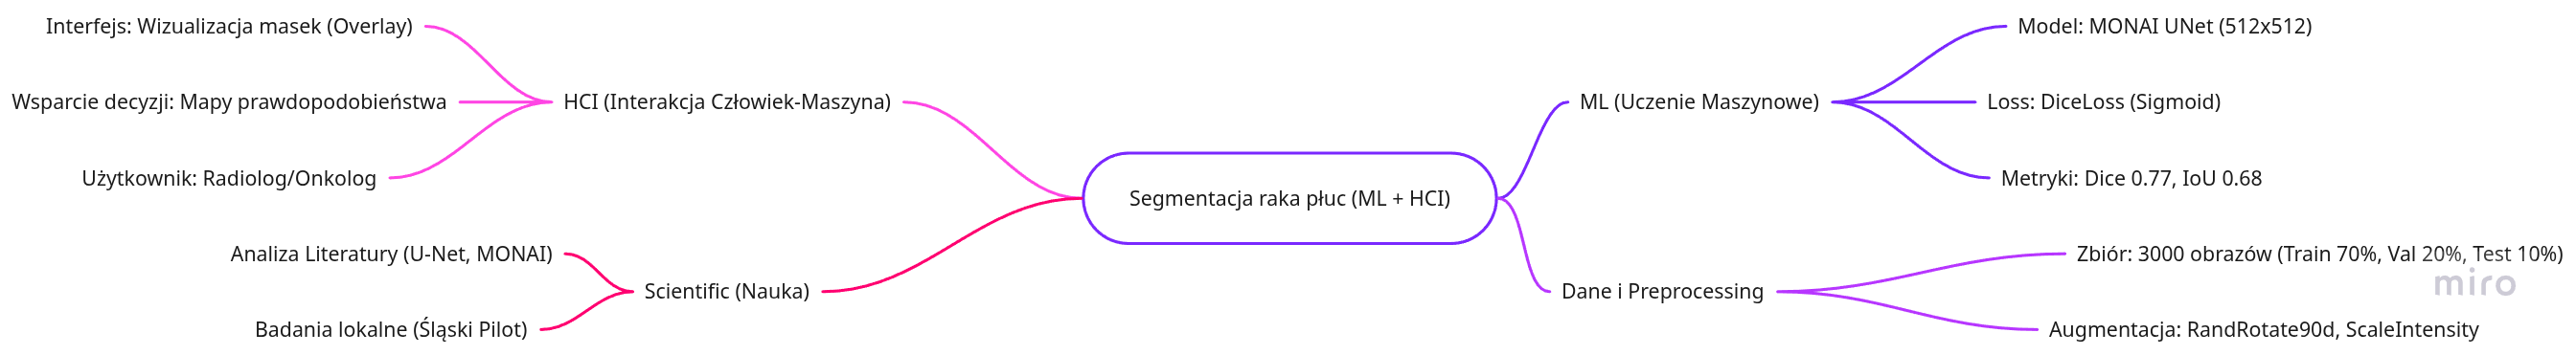
\includegraphics[width=\textwidth,height=0.3\textheight]{media/mind_map.png}
            \caption{Struktura koncepcyjna.}
        \end{figure}
\end{frame}

\begin{frame}{Zbiór danych}
    \textbf{Lung Cancer Segmentation Dataset} (Kaggle)
    \begin{itemize}
        \item \textbf{3000 par obrazów:} skany CT płuc + maski eksperckie
        \item \textbf{Format:} obrazy w skali szarości, binarne maski segmentacyjne
        \item \textbf{Podział:} 70\% trening / 20\% walidacja / 10\% test
    \end{itemize}
    \vspace{0.3cm}
    \textbf{Transformacje danych:}
    \begin{itemize}
        \item Normalizacja intensywności do zakresu [0, 1]
        \item Augmentacja: rotacja o wielokrotność $90$ (p=0.5)
    \end{itemize}
\end{frame}

\begin{frame}{Podbudowa naukowa (Scientific Attribute)}
    Wykorzystanie źródeł o charakterze naukowym
    \begin{itemize}
        \item \textbf{Architektura:} U-Net (Ronneberger et al., 2015).
        \item \textbf{Framework:} MONAI (Medical Open Network for AI).
    \end{itemize}
\end{frame}

\begin{frame}{Architektura U-Net}
    Symetryczna struktura w kształcie litery „U":
    \begin{itemize}
        \item \textbf{Encoder (ścieżka kurczenia):}
        \begin{itemize}
            \item Ekstrakcja cech przez warstwy konwolucyjne 3x3 + ReLU
            \item Max pooling 2x2 — redukcja rozdzielczości
            \item Podwajanie liczby kanałów na każdym poziomie
        \end{itemize}
        \item \textbf{Decoder (ścieżka ekspansji):}
        \begin{itemize}
            \item Up-convolution 2x2 — zwiększanie rozdzielczości
            \item Rekonstrukcja przestrzenna segmentacji
        \end{itemize}
        \item \textbf{Skip Connections:}
        \begin{itemize}
            \item Łączenie odpowiadających poziomów encoder-decoder
            \item Zachowanie szczegółów przestrzennych dla precyzyjnych granic
        \end{itemize}
    \end{itemize}
\end{frame}

\begin{frame}{Schemat architektury U-Net}
    \begin{figure}
        \centering
        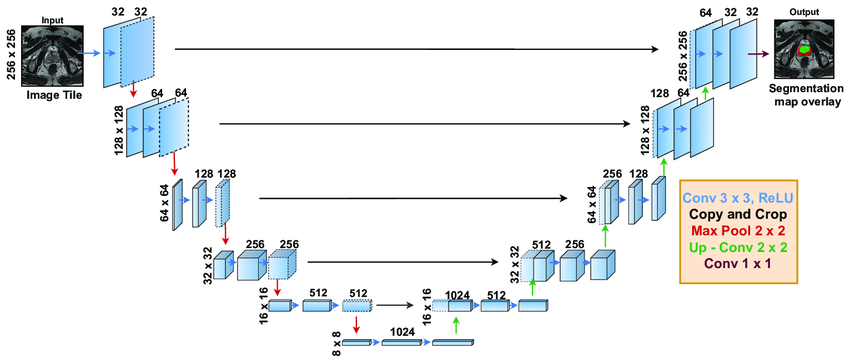
\includegraphics[width=0.8\textwidth]{./unet.png}
        \caption{Schemat architektury U-Net (Ronneberger et al., 2015).}
    \end{figure}
\end{frame}

\begin{frame}{Implementacja modelu (ML)}
    \begin{columns}
        \column{0.5\textwidth}
        \textbf{Konfiguracja MONAI UNet:}
        \begin{itemize}
            \item Wymiary: 2D
            \item Wejście/Wyjście: 1 kanał
            \item Kanały: (16, 32, 64, 128, 256)
            \item Strides: (2, 2, 2, 2)
        \end{itemize}
        \vspace{0.2cm}
        \textbf{Trening:}
        \begin{itemize}
            \item Adam ($lr=0.001$)
            \item 400 epok, batch=64
        \end{itemize}
        \column{0.5\textwidth}
        \begin{figure}
            \centering
            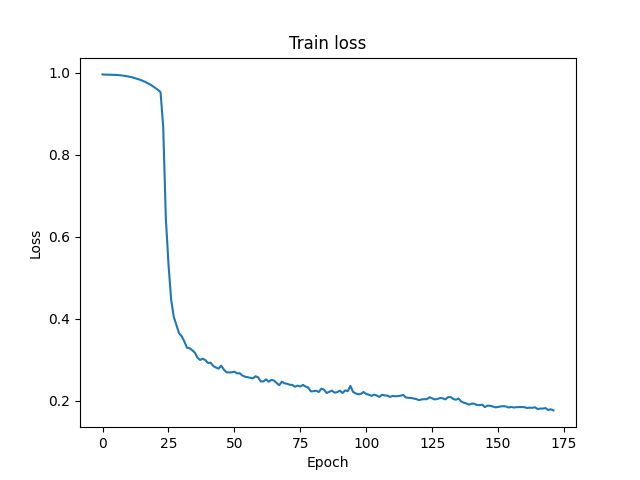
\includegraphics[width=\textwidth]{media/train_loss.png}
            \caption{Przebieg procesu uczenia.}
        \end{figure}
    \end{columns}
\end{frame}

\begin{frame}{Dice Loss — Funkcja straty}
    \textbf{Problem:} Niezrównoważenie klas — zmiany nowotworowe $\ll$ tło
    \vspace{0.3cm}

    \textbf{Rozwiązanie:} Dice Loss — odporna na niezrównoważenie klas
    \begin{equation*}
        \text{Dice Loss} = 1 - \frac{2 \sum p_i \cdot g_i + \epsilon}{\sum p_i + \sum g_i + \epsilon}
    \end{equation*}

    \vspace{0.2cm}
    \textbf{Zalety:}
    \begin{itemize}
        \item Bezpośrednia optymalizacja metryki ewaluacyjnej
        \item Lepsza konwergencja dla małych obiektów
        \item Naturalna odporność na dominację klasy tła
    \end{itemize}
\end{frame}

\begin{frame}{Metryki ewaluacji segmentacji}
    \begin{columns}
        \column{0.5\textwidth}
        \textbf{Dice Coefficient (F1-Score):}
        \begin{equation*}
            \text{Dice} = \frac{2 \cdot |P \cap G|}{|P| + |G|}
        \end{equation*}
        \begin{itemize}
            \item Mierzy podobieństwo predykcji do ground truth
            \item Zakres: [0, 1], gdzie 1 = idealne dopasowanie
        \end{itemize}

        \column{0.5\textwidth}
        \textbf{IoU (Jaccard Index):}
        \begin{equation*}
            \text{IoU} = \frac{|P \cap G|}{|P \cup G|}
        \end{equation*}
        \begin{itemize}
            \item Stosunek części wspólnej do sumy zbiorów
            \item Bardziej rygorystyczna niż Dice
        \end{itemize}
    \end{columns}
    \vspace{0.3cm}
    \textbf{Relacja:} $\text{Dice} = \frac{2 \cdot \text{IoU}}{1 + \text{IoU}}$ — Dice $\geq$ IoU
\end{frame}

\begin{frame}{Wyniki ilościowe}
    Ewaluacja na zbiorze testowym (300 obrazów = 10\% zbioru):
    \begin{table}
        \centering
        \begin{tabular}{|l|c|l|}
            \hline
            \textbf{Metryka} & \textbf{Wartość} & \textbf{Interpretacja} \\
            \hline
            Dice Coefficient & \textbf{0.77} & Dobra zgodność segmentacji \\
            \hline
            IoU (Jaccard) & 0.68 & Solidne pokrycie zmian \\
            \hline
            Recall (Czułość) & 0.80 & Wysoka czułość diagnostyczna \\
            \hline
            Precision & 0.78 & Niski poziom fałszywych alarmów \\
            \hline
        \end{tabular}
    \end{table}
    \vspace{0.2cm}
    \textbf{Wniosek:} Wysoki Recall (0.80) jest kluczowy w diagnostyce medycznej — minimalizacja pominięć zmian nowotworowych.
\end{frame}

\begin{frame}{System interakcji (HCI)}
    \begin{itemize}
        \item Interaktywne wgrywanie plików.
        \item Wizualizacja masek i Probability Maps.
    \end{itemize}
    \begin{figure}
        \centering
        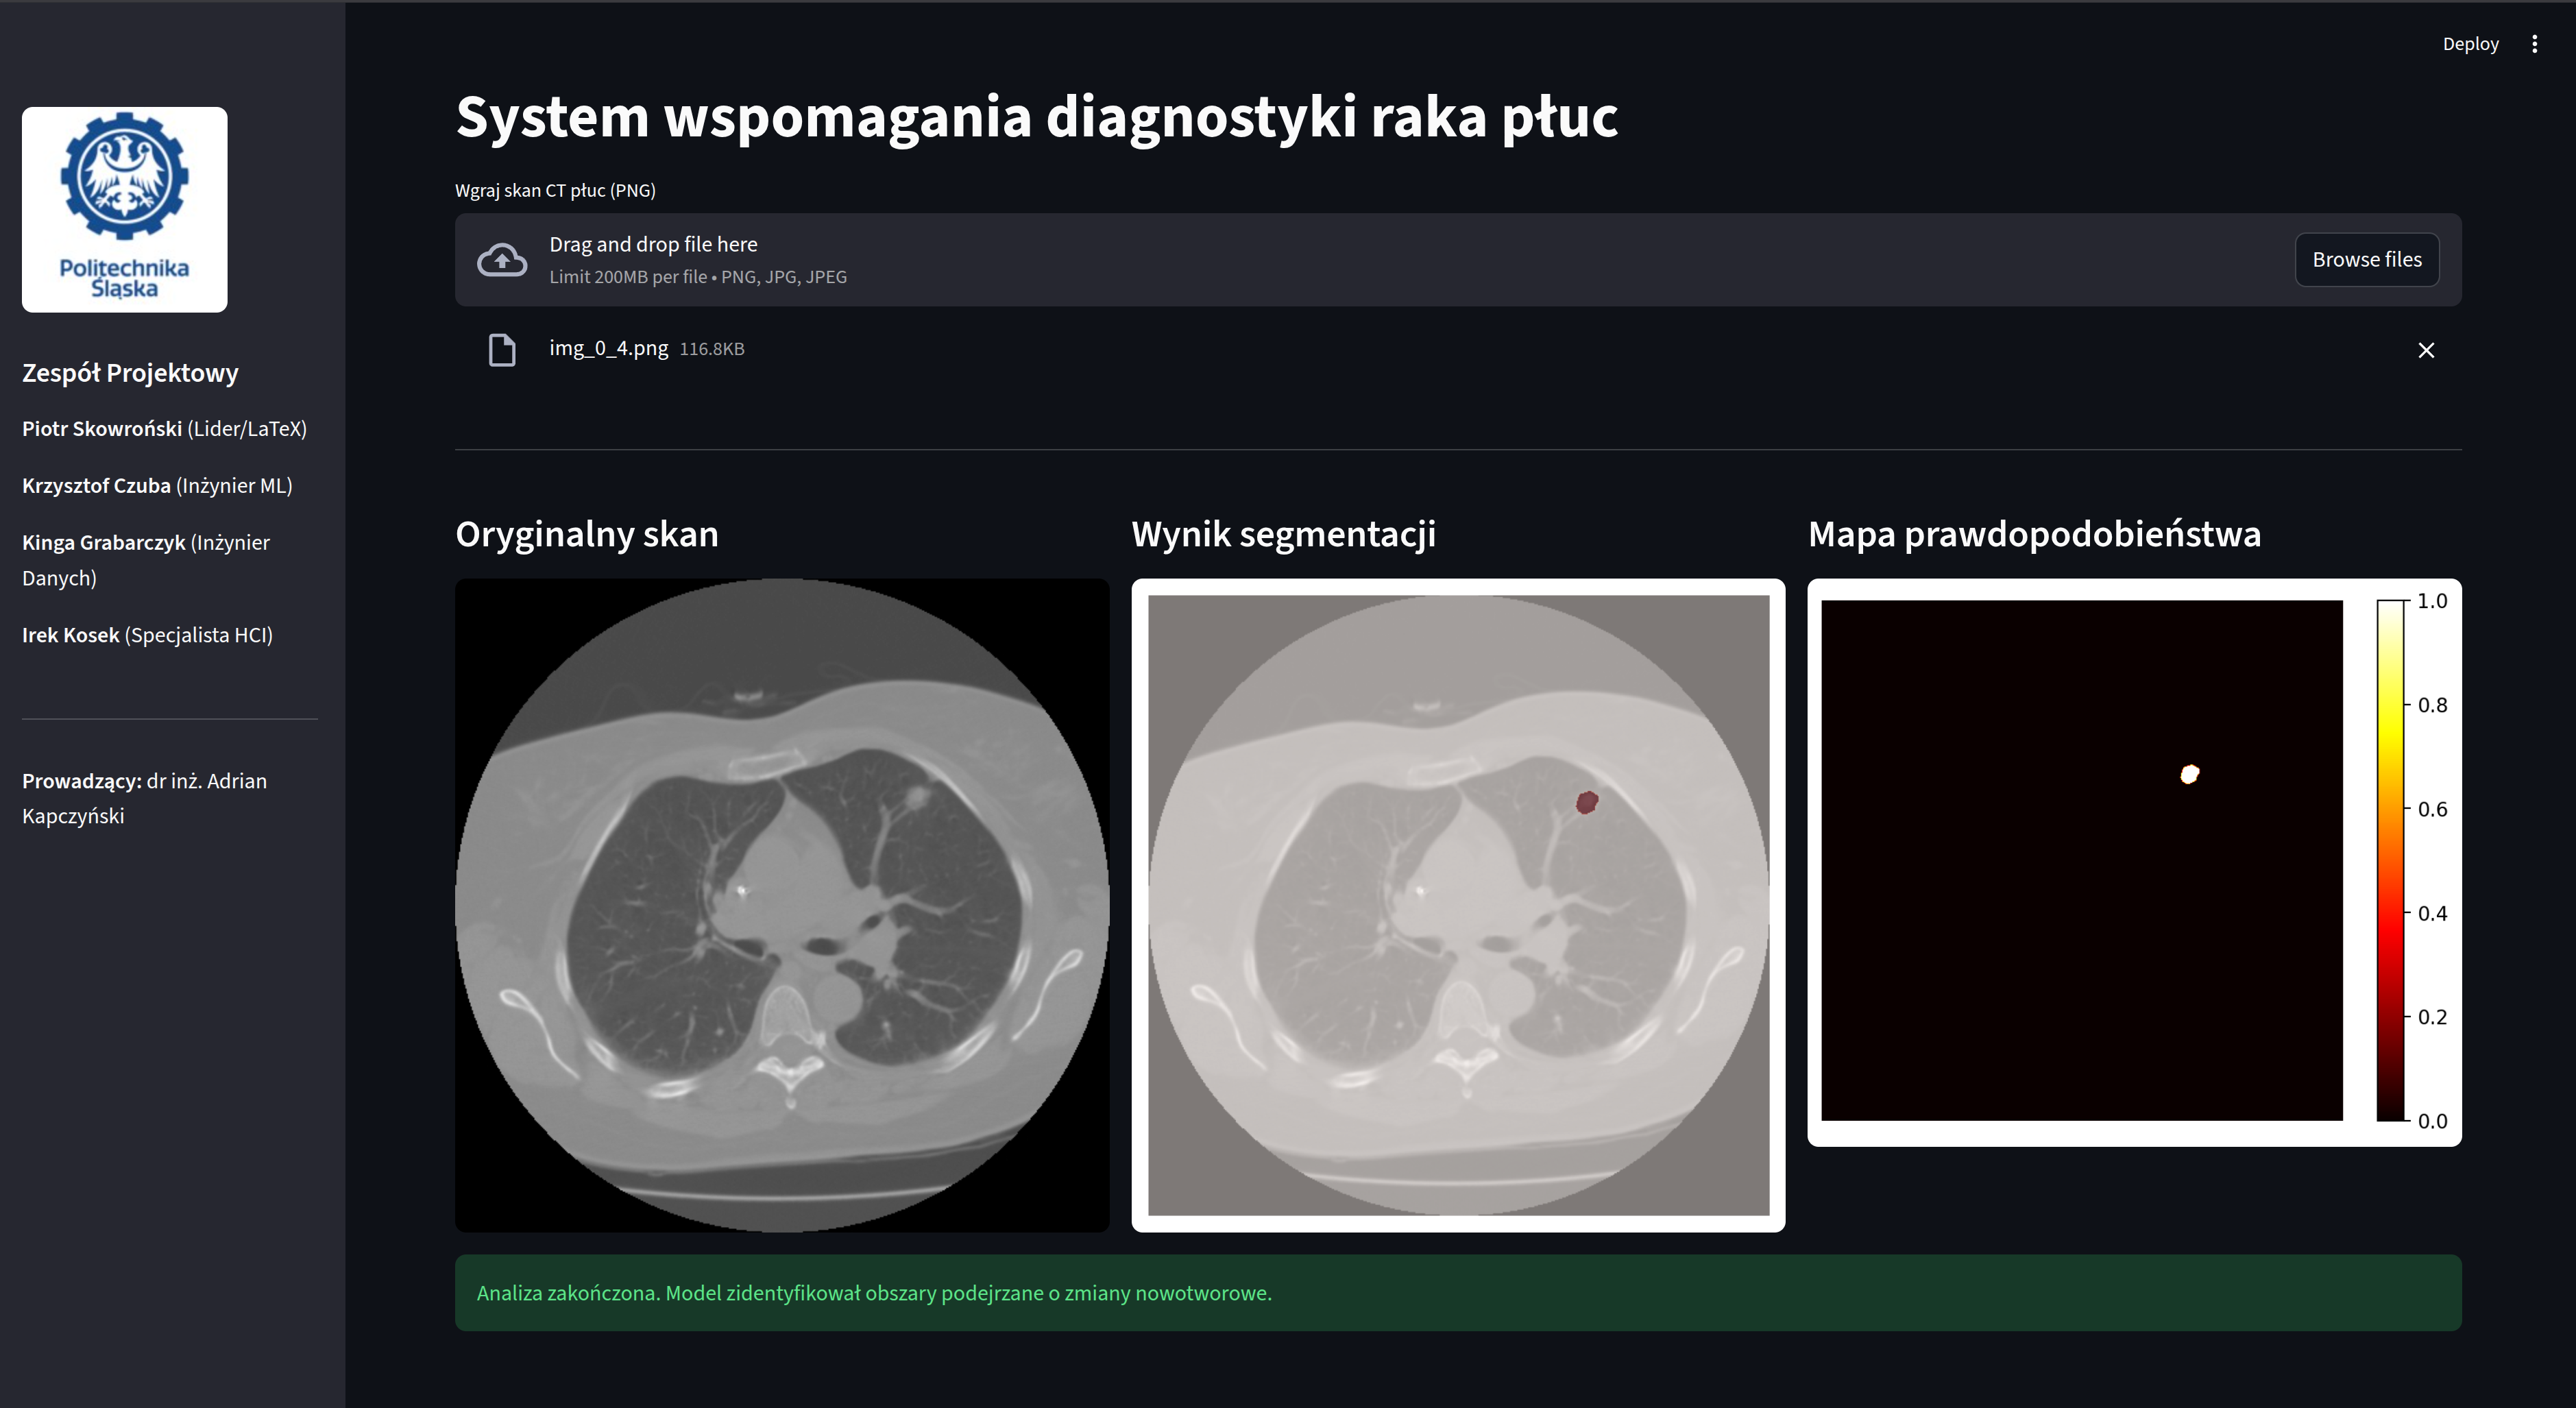
\includegraphics[width=0.7\textwidth]{media/app_screenshot.png}
        \caption{Interfejs systemu wspomagania diagnostyki.}
    \end{figure}
\end{frame}

\begin{frame}{Wizualizacja wyników segmentacji}
    \begin{figure}
        \centering
        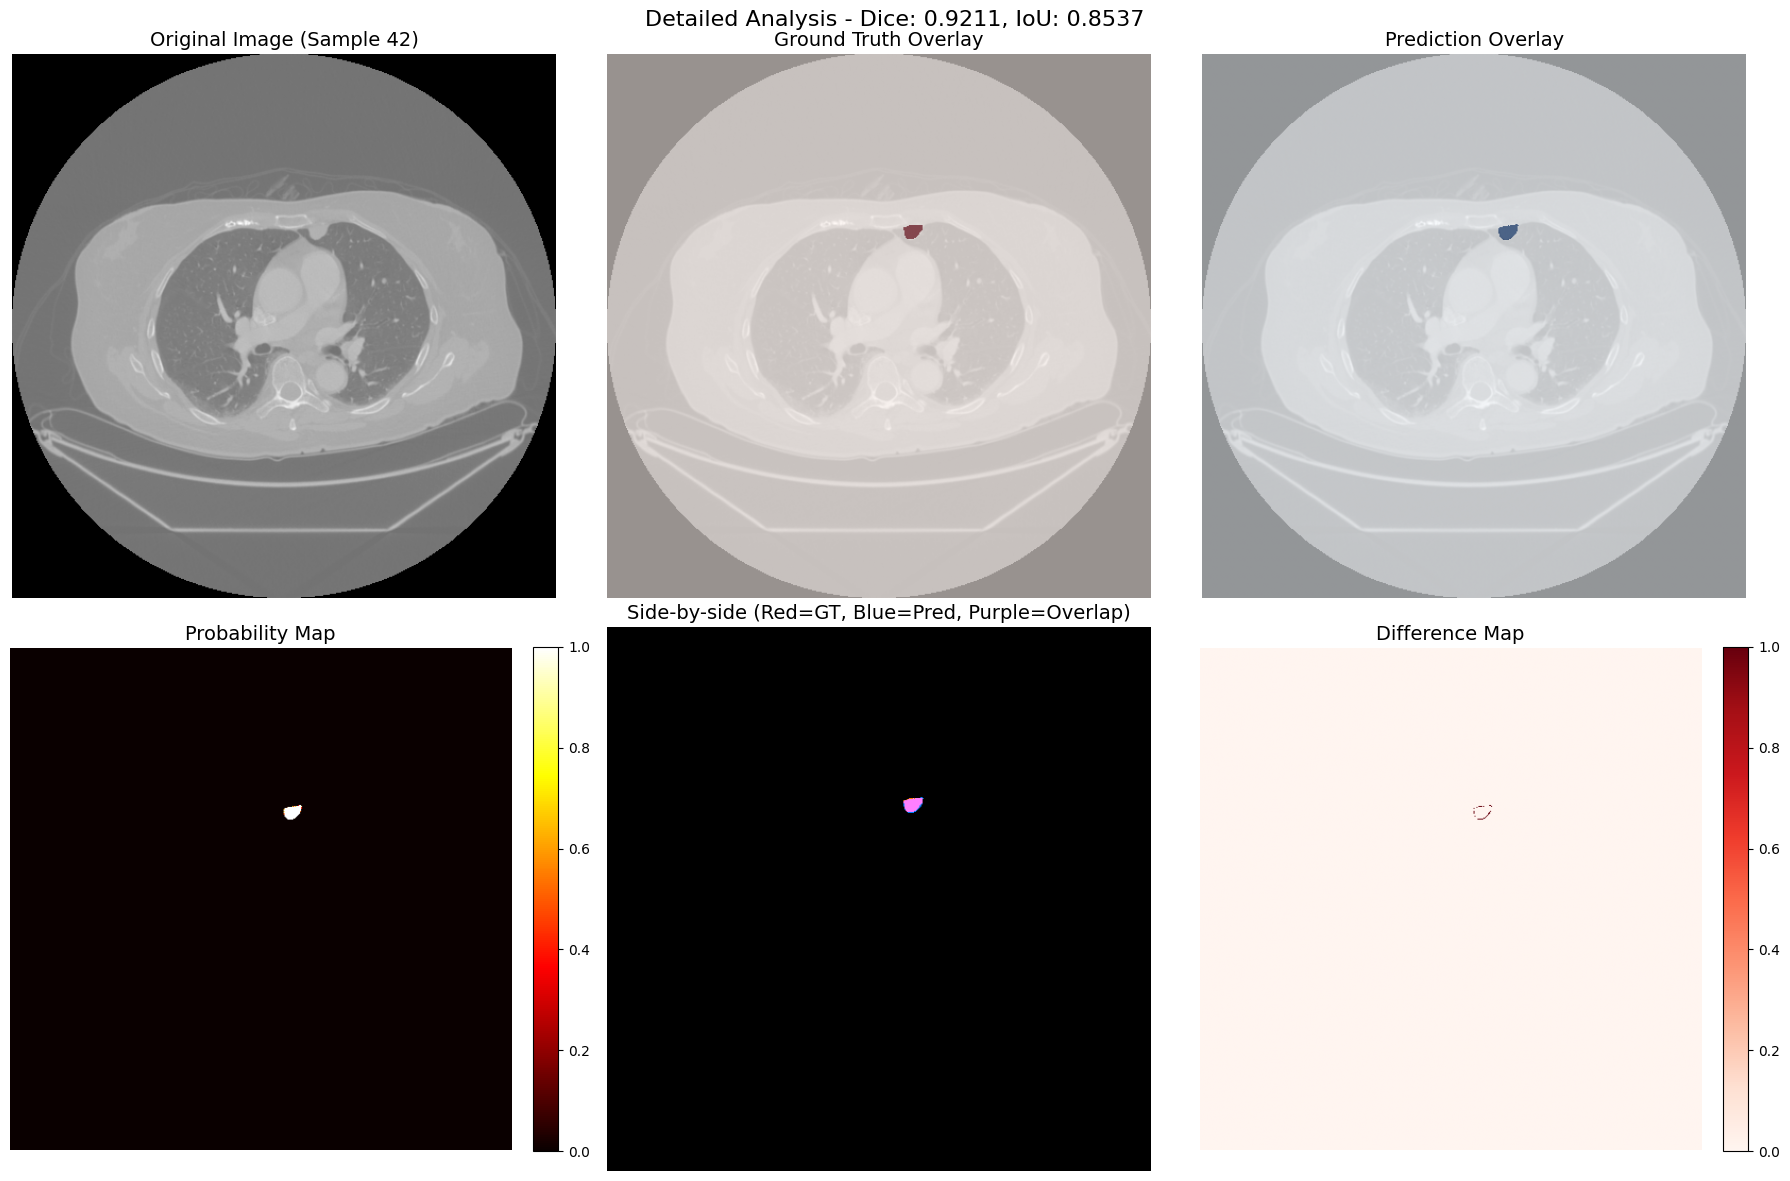
\includegraphics[width=0.9\textwidth]{media/model_predictions_comparison.png}
        \caption{Porównanie: Oryginał vs Ground Truth vs Predykcja.}
    \end{figure}
\end{frame}


\begin{frame}{Podsumowanie}
    \begin{itemize}
        \item Opracowano kompletny scenariusz diagnostyczny.
        \item Zintegrowano zaawansowane ML z interfejsem wspierającym lekarza.
    \end{itemize}
    \vspace{1cm}
\end{frame}

\end{document}
